\section{Versuchsaufbau}
\label{sec:Versuchsaufbau}
Die wichigsten Bausteine dieses Versuches sind der Lautsprecher und das Mikrofon, sowie 
die damit verbunden Steuerelektronik. Sie werden für jeden Versuchsteil benötigt.
Innerhalb dieser Steuerelektronik befindet sich ein Frequenz-Spannungskonverter, 
der es ermöglicht Frequenzspektren auf einem Oszilloskop oder COmputer zu visualisieren.
Auf dem Computer erfolgt die Darstellung mit dem Programm SpectrumSLC.
Der Lautsprecher ist mit einem Sinusgenreator verbunden, üder den die passenden 
Frequenzen erzeugt werden können.

Für unterschiedliche Versuchsteile werden verschiedene Hohlraumresonatoren benötigt:
\begin{itemize}
    \item 1-dim Festkörper:
        \begin{itemize}
            \item Aluminiumzylinder der Längen:
                \begin{itemize}
                    \item $\SI{12,5}{\milli\meter}$ 
                    \item $\SI{50}{\milli\meter}$
                    \item $\SI{75}{\milli\meter}$
                \end{itemize}
            \item Blenden der Durchmesser:
                \begin{itemize}
                    \item $\SI{10}{\milli\meter}$
                    \item $\SI{13}{\milli\meter}$
                    \item $\SI{16}{\milli\meter}$
                \end{itemize}
        \end{itemize}
    \item Wasserstoffatom:
        \begin{itemize}
            \item Kugelresonator aus zwei Halbkugeln
            \item Mikrofon in einer Halbkugel, $\SI{45}{\degree}$ relativ zur Horizontalen eingebaut
            \item Lautsprecher in der anderen Halbkugel, $\SI{45}{\degree}$ relativ zur Horizontalen, $\SI{180}{\degree}$ relativ zum Mikrofon eingebaut
            \item zwei Ringe ($\SI{3}{\milli\meter}$ und $\SI{9}{\milli\meter}$ Dicke) die zwischen die Halbkugeln geschraubt werden können
        \end{itemize}
    \item Wasserstoffmolekül:
        \begin{itemize}
            \item Kugelresonator aus zwei Halbkugeln wie beim Wasserstoffatom
            \item zwei weitere Halbkugeln mit je einer Öffnung
            \item zwei Blenden ($\SI{10}{\milli\meter}$ und $\SI{16}{\milli\meter}$ Durchmesser), die zwischen den Kugeln befestigt werden können
        \end{itemize}
\end{itemize}

\begin{figure}
    \centering
    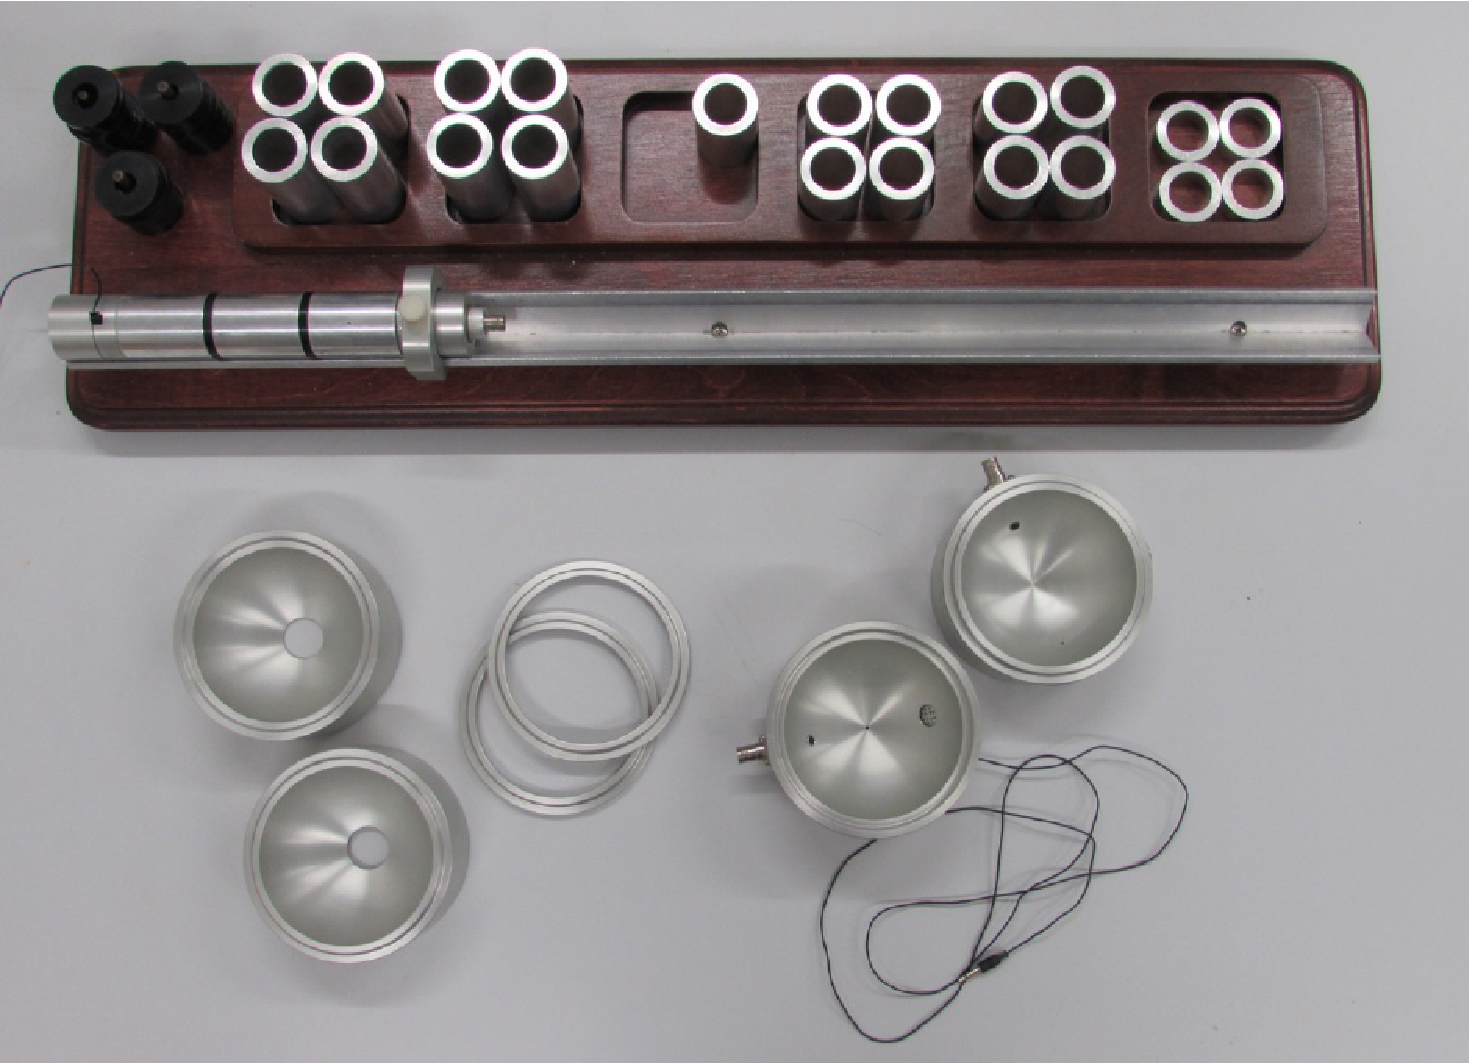
\includegraphics[width=0.8\textwidth]{figure/Aufbau.pdf}
    \caption{
            In dieser Abbildung sind die Baukomponenten der einzelnen Versuchsteile 
            dargestellt. Im oberen Bildbereich sind die Aluminumzylinder und die 
            zugehörigen schwarzen Blenden zu sehen. Direkt darunter befindet sich die 
            Metallschiene auf der die Zylinder aufgereiht und zur Frequenzmessung 
            positioniert werden können. Im unteren Bildbereich sind rechts die beiden 
            Hälften des Kugelresonators mit Lautsprecher und Mikrofon, mittig die 
            Zwischenringe und links die beiden Halbkugeln mit Öffnungen abgebildet 
            \cite{sample}.
            }
\end{figure}




\section{Versuchsdurchführung}
\label{sec:Versuchsdurchführung}
